% =============================================================================
%  MOZU — Test plan for the scan-to-design pipeline
%  Technical report MOZU-TP-001, version 1.0
%
%  Build:  pdflatex mozu-test-plan.tex   (run twice for cross-references)
%  Needs:  IEEEtran, TikZ, pgfgantt, booktabs, tabularx, longtable, listings
%          (all in TeX Live / MacTeX / Overleaf by default)
%
%  Deliberately black and white: owners are told apart by fill pattern
%  (solid / hatched / outline), never by colour, so the document prints and
%  photocopies without losing information.
% =============================================================================
\documentclass[conference,a4paper,10pt]{IEEEtran}
\IEEEoverridecommandlockouts

\usepackage{cite}
\usepackage{amsmath,amssymb}
\usepackage{booktabs}
\usepackage{array}
\usepackage{tabularx}
\usepackage{longtable}
\usepackage{multirow}
\usepackage{listings}
\usepackage{tikz}
\usetikzlibrary{arrows.meta,positioning,patterns,calc,fit}
\usepackage{pgfgantt}
\usepackage[hyphens]{url}
\usepackage[hidelinks]{hyperref}

% ---- Float placement ----------------------------------------------------------
% Let full-width figures and tables take most of a page (or a page of their
% own) rather than leaving a stray line or two of text beneath them.
\renewcommand{\topfraction}{0.9}
\renewcommand{\dbltopfraction}{0.95}
\renewcommand{\textfraction}{0.08}
\renewcommand{\floatpagefraction}{0.8}
\renewcommand{\dblfloatpagefraction}{0.8}

% ---- Tables -----------------------------------------------------------------
\newcolumntype{L}[1]{>{\raggedright\arraybackslash}p{#1}}
\newcolumntype{C}[1]{>{\centering\arraybackslash}p{#1}}
\newcolumntype{Y}{>{\raggedright\arraybackslash}X}
\renewcommand{\arraystretch}{1.12}

% ---- Small helpers ------------------------------------------------------------
\newcommand{\code}[1]{\path{#1}}
\newcommand{\swts}{Swift\,$\leftrightarrows$\,TypeScript}
\newcommand{\req}{$\bullet$}

% ---- Listings: plain, black and white ------------------------------------------
\lstset{
  basicstyle=\ttfamily\footnotesize,
  columns=fullflexible,
  keepspaces=true,
  frame=single,
  framerule=0.4pt,
  breaklines=true,
  showstringspaces=false,
  xleftmargin=4pt,
  xrightmargin=4pt,
}

\begin{document}

\title{Verifying a LiDAR Scan-to-Design Pipeline:\\
A Test Plan for MOZU with Division of Work\\ and a Four-Week Schedule%
\thanks{Technical Report MOZU-TP-001, version 1.0, 1 October 2026.
Baseline under test: repository \texttt{cosmosmining/mozu-configurator},
commit \texttt{02784c8}. The operational checklist that accompanies this plan
is \texttt{docs/TESTING-PLAN.md} in the same repository.}}

\author{%
\IEEEauthorblockN{Johnson}
\IEEEauthorblockA{\textit{Scanning lead; editor of this plan}\\
iPad capture, LiDAR, field campaign\\
MOZU}
\and
\IEEEauthorblockN{Avery}
\IEEEauthorblockA{\textit{Backend lead}\\
Handoff service, scan SDK, CI\\
MOZU}
\and
\IEEEauthorblockN{Alvin}
\IEEEauthorblockA{\textit{Front-end lead}\\
3D scene, models, placement\\
MOZU}}

\maketitle

% =============================================================================
\begin{abstract}
MOZU couples an iPad scanner, built on Apple RoomPlan and the device's LiDAR
depth sensor, with a web-based room configurator. A scan becomes a dimensioned
floor plan carrying doors, windows, columns and power sockets, and is handed
to the web through a six-character code. Early field tests exposed four
classes of failure: glass that was not detected, light fixtures reported as
sockets, clutter that displaced walls, and round columns that corrupted the
room outline. This paper specifies how the corrected system will be verified
between 5 and 30 October 2026 by a team of three: Johnson (scanning), Avery
(backend) and Alvin (front end). The strategy combines six automated
layers---unit tests, property-based fuzzing against generated ground truth,
differential testing between the Swift and TypeScript implementations,
golden-scan regression, browser end-to-end tests and a full device
build---with a ground-truthed field protocol scored against quantitative
acceptance limits. Preliminary results show that fuzzing exposed incorrect
outlines in 278 of 1{,}000 generated rooms in the previous build and in none
in the current one, and that the two implementations agree on 2{,}000 rooms
within a relative tolerance of $10^{-6}$. Accuracy on real devices has not yet
been measured; it is the subject of the first two weeks of the plan.
\end{abstract}

\begin{IEEEkeywords}
software testing, test planning, LiDAR, RoomPlan, floor-plan reconstruction,
property-based testing, differential testing, end-to-end testing
\end{IEEEkeywords}

% =============================================================================
\section{Introduction}

A fitted kitchen is designed around the room it will stand in, so the room
has to be measured before anything else can happen. MOZU replaces the tape
measure with an iPad scan. Apple's RoomPlan framework~\cite{roomplan}
reconstructs walls, doors, windows and large objects from the LiDAR depth
stream~\cite{ardepth}. MOZU adds three analyses of its own: a \emph{wall
analysis} that removes clutter and columns from the outline, a \emph{glass
finder} that detects panes RoomPlan did not recognise, and a \emph{socket
detector} that locates power outlets on the walls. The finished scan is
uploaded, and the iPad displays a six-character code. Entering the code on a
laptop opens the room in a web configurator, where cabinets and furniture are
placed in two and three dimensions.

Field testing of early builds surfaced four defects, summarised in
Table~\ref{tab:defects}. Glass sliding doors and full-height panes were not
detected. LED strip lights were reported as sockets, and the markers appeared
to wander. Shoes and boxes standing along a wall pulled that wall into the
room. Round columns produced a spike across the plan. Each defect has been
addressed in code, but none has yet been confirmed on a device.

This document is the plan for that confirmation and for the release candidate
that follows. It covers the elements required by IEEE~829~\cite{ieee829} and
ISO/IEC/IEEE~29119-3~\cite{iso29119}: test items, features, approach,
pass/fail criteria, environment, responsibilities, schedule and risks. It is
written as a paper so that the reasoning behind each decision is recorded
alongside the decision. Its contributions are:

\begin{itemize}
\item quantitative acceptance criteria (Section~\ref{sec:criteria}) enforced
  by a scoring tool, which turn manual tests into measurements;
\item a layered automated strategy (Section~\ref{sec:method}) in which
  generated ground truth and differential testing compensate for the absence
  of LiDAR hardware in continuous integration;
\item a ground-truthed field protocol, with a sample-size argument for socket
  recall (Section~\ref{sec:field});
\item an explicit division of work across three owners, with interface
  contracts and a responsibility matrix (Section~\ref{sec:team}); and
\item a four-week schedule with milestones and go/no-go criteria
  (Section~\ref{sec:schedule}).
\end{itemize}

Section~\ref{sec:sut} describes the system under test.
Section~\ref{sec:team} assigns the work. Sections~\ref{sec:method}
to~\ref{sec:criteria} define the method, the environment and the pass
criteria. Sections~\ref{sec:schedule} to~\ref{sec:defects} cover the
schedule, the risks and defect handling. Section~\ref{sec:results} reports
the evidence available at the baseline, and Section~\ref{sec:conclusion}
concludes. Appendix~\ref{app:cases} lists every test case by owner.

% =============================================================================
\section{System Under Test}\label{sec:sut}

\subsection{Architecture}

The system has three subsystems joined by two data contracts
(Fig.~\ref{fig:arch}). The iPad produces a \emph{RoomScan} document (schema
\texttt{mozu.roomscan/1}). The backend stores it under a short code for
24~hours. The web front end retrieves it by code and converts it into its own
room model. Ownership follows the subsystem boundaries: each subsystem has one
owner, who also owns its test evidence.

\begin{figure*}[!t]
\centering
\resizebox{\textwidth}{!}{%
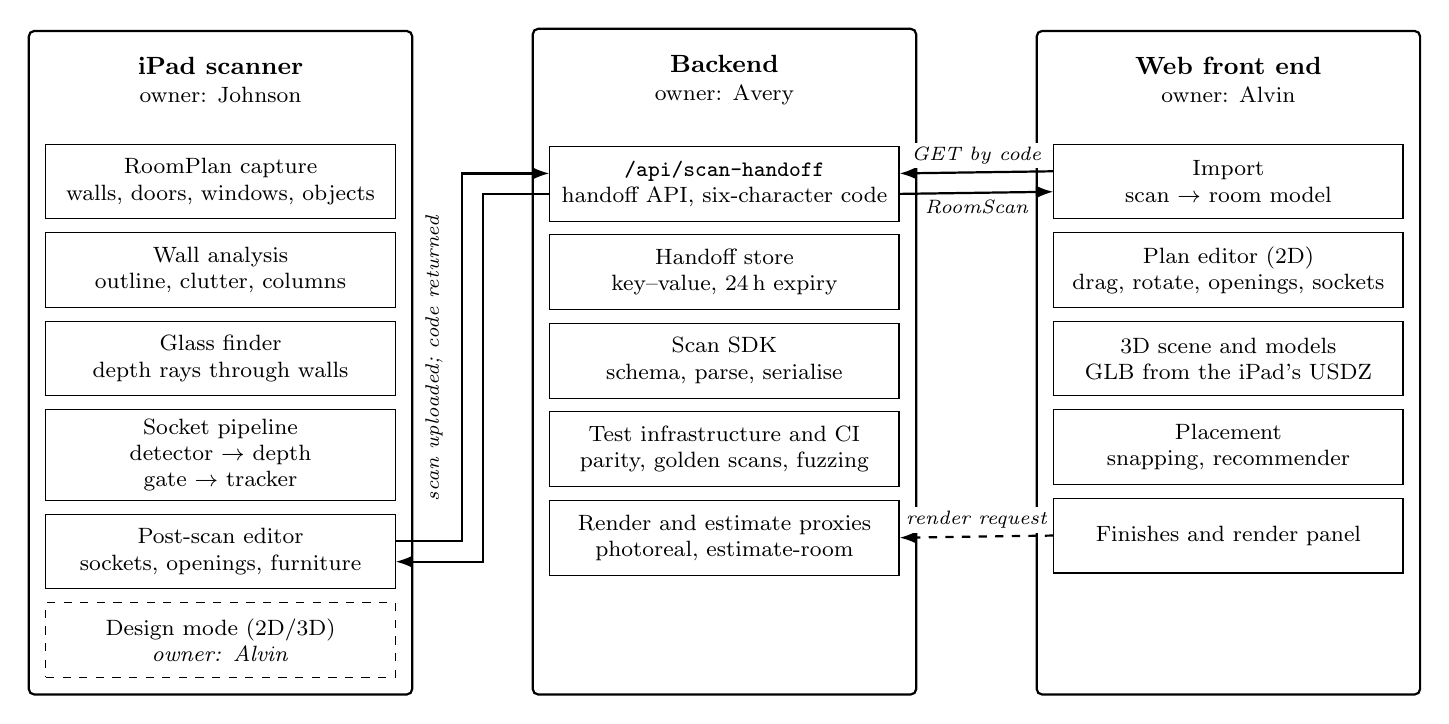
\begin{tikzpicture}[
  font=\footnotesize,
  sub/.style={draw, thick, rounded corners=2pt, inner sep=6pt},
  item/.style={draw, fill=white, minimum width=4.4cm, minimum height=0.95cm,
               align=center, text width=4.2cm},
  head/.style={font=\small\bfseries, align=center},
  flow/.style={-{Latex[length=2.2mm]}, thick},
  lbl/.style={font=\scriptsize\itshape, align=center, fill=white, inner sep=1.5pt},
]
% Every box has the same height, so rows line up across the three columns and
% the arrows between them run straight.
% --- iPad (Johnson) ---
\node[head] (h1) at (0,0) {iPad scanner\\[-1pt]\normalfont\footnotesize owner: Johnson};
\node[item, below=4mm of h1] (a1) {RoomPlan capture\\ walls, doors, windows, objects};
\node[item, below=1.6mm of a1] (a2) {Wall analysis\\ outline, clutter, columns};
\node[item, below=1.6mm of a2] (a3) {Glass finder\\ depth rays through walls};
\node[item, below=1.6mm of a3] (a4) {Socket pipeline\\ detector $\rightarrow$ depth gate $\rightarrow$ tracker};
\node[item, below=1.6mm of a4] (a5) {Post-scan editor\\ sockets, openings, furniture};
\node[item, below=1.6mm of a5, dashed] (a6) {Design mode (2D/3D)\\ \textit{owner: Alvin}};
\node[sub, fit=(h1)(a1)(a6)] (ipad) {};

% --- Backend (Avery) ---
\node[head] (h2) at (6.4,0) {Backend\\[-1pt]\normalfont\footnotesize owner: Avery};
\node[item, below=4mm of h2] (b1) {\texttt{/api/scan-handoff}\\ handoff API, six-character code};
\node[item, below=1.6mm of b1] (b2) {Handoff store\\ key--value, 24\,h expiry};
\node[item, below=1.6mm of b2] (b3) {Scan SDK\\ schema, parse, serialise};
\node[item, below=1.6mm of b3] (b4) {Test infrastructure and CI\\ parity, golden scans, fuzzing};
\node[item, below=1.6mm of b4] (b5) {Render and estimate proxies\\ photoreal, estimate-room};
\node[sub, fit=(h2)(b1)(b5)(b5.south |- a6.south)] (back) {};

% --- Web (Alvin) ---
\node[head] (h3) at (12.8,0) {Web front end\\[-1pt]\normalfont\footnotesize owner: Alvin};
\node[item, below=4mm of h3] (c1) {Import\\ scan $\rightarrow$ room model};
\node[item, below=1.6mm of c1] (c2) {Plan editor (2D)\\ drag, rotate, openings, sockets};
\node[item, below=1.6mm of c2] (c3) {3D scene and models\\ GLB from the iPad's USDZ};
\node[item, below=1.6mm of c3] (c4) {Placement\\ snapping, recommender};
\node[item, below=1.6mm of c4] (c5) {Finishes and render panel};
\node[sub, fit=(h3)(c1)(c5)(c5.south |- a6.south)] (web) {};

% --- Flows ---
% Mid-lines in the gaps between the subsystems, for routing.
\path (ipad.east) -- (back.west) coordinate[pos=0.5] (g1);
% iPad -> backend: the scan goes up; the code comes back.
% The return route runs to the right of the outgoing one, so they never cross.
\draw[flow] ([yshift=1.3mm]a5.east) -- ([xshift=-1.3mm,yshift=1.3mm]a5.east -| g1)
  |- ([yshift=1.3mm]b1.west);
\draw[flow] ([yshift=-1.3mm]b1.west) -- ([xshift=1.3mm,yshift=-1.3mm]b1.west -| g1)
  |- ([yshift=-1.3mm]a5.east);
\node[lbl, rotate=90, anchor=south] at ($(a3.east -| g1)+(-3.2mm,0)$)
  {scan uploaded; code returned};
% Web <-> backend: the code goes in; the scan comes back.
\draw[flow] ([yshift=1.3mm]c1.west) -- node[lbl, above=1pt] {GET by code} ([yshift=1.3mm]b1.east);
\draw[flow] ([yshift=-1.3mm]b1.east) -- node[lbl, below=1pt] {RoomScan} ([yshift=-1.3mm]c1.west);
% Web -> render proxy.
\draw[flow, dashed] (c5.west) -- node[lbl, above=1pt] {render request} (b5.east);
\end{tikzpicture}}
\caption{System under test. Solid boxes are components; arrows are the data
contracts between subsystems (Section~\ref{sec:contracts}). The iPad's design
mode is drawn dashed because it runs on the iPad but belongs to the front-end
workstream.}
\label{fig:arch}
\end{figure*}

\subsection{Components and ownership}

Table~\ref{tab:components} maps each component to its implementation, owner
and principal verification. Several components exist twice: once in Swift on
the iPad and once in TypeScript, where most of the tests are written. The
correspondence between these twins is itself tested
(Section~\ref{sec:differential}).

\begin{table*}[!t]
\caption{Components, Implementation, Owner and Principal Verification}
\label{tab:components}
\centering
\footnotesize
\begin{tabularx}{\textwidth}{@{}L{3.6cm}YL{1.3cm}L{4.3cm}@{}}
\toprule
Component & Implementation (repository paths) & Owner & Verified by \\
\midrule
Room capture and export & \code{apps/ios/.../Scan/RoomCaptureController.swift}, \code{FloorplanBuilder.swift} & Johnson & device build; field \\
Wall analysis (outline, clutter, columns) & \code{Scan/WallLoop.swift} $\leftrightarrows$ \code{src/systems/scan/wallLoop.ts} & Johnson & unit; fuzzing; differential; field \\
Glass finder & \code{Scan/GlassFinder.swift} $\leftrightarrows$ \code{glassFinder.ts} & Johnson & unit; differential; field \\
Socket pipeline & \code{SocketDetector}, \code{DepthGate}, \code{FixtureCapture} $\leftrightarrows$ \code{fixtureDetector.ts}, \code{plateGeometry.ts} & Johnson & unit; differential (detector); field \\
Post-scan editor & \code{Views/FloorplanResultView.swift} & Johnson & device; field \\
\midrule
Handoff API and store & \code{src/app/api/scan-handoff}, \code{src/systems/handoff} & Avery & API tests; end-to-end \\
Scan schema and SDK & \code{packages/scan-sdk} & Avery & unit; golden scans \\
Render and estimate proxies & \code{src/app/api/photoreal}, \code{src/app/api/estimate-room} & Avery & API tests \\
Test infrastructure and CI & \code{.github/workflows/ci.yml}, \code{apps/ios/ParityHarness}, \code{scripts/scan-accuracy.mjs}, \code{fixtures/scans} & Avery & CI \\
\midrule
Import and room model & \code{src/systems/scan/scanToGeometry.ts}, \code{src/state/slices} & Alvin & golden scans; end-to-end \\
Plan editor (2D) & \code{src/components/room/PlanEditor.tsx} & Alvin & end-to-end; visual regression \\
3D scene, models, lighting & \code{src/three}, \code{public/models}, \code{scripts/usdz-to-glb.py} & Alvin & end-to-end; visual; model audit \\
Placement, recommender, finishes & \code{src/systems/layout}, \code{furniture}, \code{aesthetic} & Alvin & unit; end-to-end \\
iPad design mode & \code{apps/ios/.../Design} & Alvin & device; comparison with web \\
\bottomrule
\end{tabularx}
\end{table*}

\subsection{Field defects}

Table~\ref{tab:defects} records the defects reported from the field, their
root causes and the tests that will confirm each fix.

\begin{table}[!t]
\caption{Field Defects, Causes and Confirming Tests}
\label{tab:defects}
\centering
\footnotesize
\begin{tabularx}{\columnwidth}{@{}L{1.5cm}YL{1.35cm}@{}}
\toprule
Report & Root cause and remedy & Confirmed by \\
\midrule
Glass not detected &
RoomPlan recognises framed windows only. Depth readings pass \emph{through}
clear glass; the glass finder treats walls the sensor saw through as
suggested openings, which the user keeps or removes. &
\mbox{GLS-01--04} \\
LED lights taken for sockets; markers wander &
Light sources clip the sensor; candidates that are both clipped and brighter
than any reflector are rejected. The marker overlay was redrawn at 5\,Hz and
is now redrawn every frame. &
\mbox{SKT-02--04} \\
Shoes move walls &
Fragments were averaged and chained by far endpoint. The outermost fragment
is now kept; low surfaces in front of walls are discarded. &
\mbox{SCN-04--05} \\
Round column spike &
Column facets were chained into the outline. They are now extracted and
fitted as a circle~\cite{kasa} or box. &
\mbox{COL-01--04} \\
Detection too slow &
Debug builds compiled without optimisation (3{,}208\,ms per frame);
optimisation is now enabled. &
PRF-01 \\
\bottomrule
\end{tabularx}
\end{table}

% =============================================================================
\section{Team Organisation and Division of Work}\label{sec:team}

Three people share the work, and each owns one subsystem end to end: its
code, its tests, its defects and the evidence that it meets the criteria.
Ownership does not mean exclusivity. Every change is reviewed by a second
member, and a change to a shared contract is reviewed by both other members.
Cross-cutting activities are allocated in the responsibility matrix,
Table~\ref{tab:raci}.

\subsection{Johnson --- scanning lead}

\textbf{Scope.} The iPad capture pipeline, from the RoomPlan session to the
RoomScan document: wall analysis, columns, glass finder, socket detection and
tracking, the post-scan editor, and on-device performance. This covers the
Swift code and the TypeScript twins of the same algorithms. Johnson also runs
the field campaign, edits this plan, chairs the go/no-go review and compiles
the weekly report.

\textbf{Responsibilities.}
\begin{itemize}
\item Plan and run the field campaign (Section~\ref{sec:field}): measure
  ground truth, scan every room three times, score every scan, and file
  defects with the scan file attached.
\item Own test cases SCN, COL, GLS, OPN, SKT, FUR, PRF and DEV
  (Appendix~\ref{app:johnson}).
\item Add the raw-surface export, so that a wall defect found in the field
  can be replayed as an automated test, and an XCTest target for the
  platform-independent Swift code.
\item Tune the socket detector on images captured in the field, keeping the
  Swift and TypeScript detectors identical.
\item Record detection time for every scan on every device.
\end{itemize}

\textbf{Deliverables.} Field log; at least 45 scored scans; a scan corpus with
ground truth; the weekly accuracy report.

\subsection{Avery --- backend lead}

\textbf{Scope.} The services and data between the iPad and the web: the
handoff API and store, the RoomScan schema and scan SDK, the render and
estimate proxies, the continuous-integration pipeline and the shared test
infrastructure (golden scans, parity harness, scoring tool). This includes
staging and production deployment of the handoff.

\textbf{Responsibilities.}
\begin{itemize}
\item Own test cases API, SDK, GLD, REN, EST, CI, SEC and LOAD
  (Appendix~\ref{app:avery}).
\item Bring up CI with all four jobs, keep it green, and alert on nightly
  fuzzing regressions.
\item Stand up a staging environment with a shared key--value store, and
  verify multi-instance behaviour, expiry and every error path.
\item Curate the golden-scan corpus: ingest each scored field scan within one
  working day and review every snapshot change.
\item Assess abuse and privacy: payload limits, code guessing, 24-hour
  retention.
\item Load-test the handoff, and confirm that long renders survive the
  proxy and hosting timeouts.
\end{itemize}

\textbf{Deliverables.} Green CI; staging environment; API test suite; golden
corpus of at least ten real rooms; load-test report; production deployment
checklist.

\subsection{Alvin --- front-end lead}

\textbf{Scope.} Everything the user sees after entering the code: the import
into the room model, the 2D plan editor, the 3D scene and lighting, the
furniture models (converted to GLB from the iPad's USDZ files), placement
(drag, rotate, snap, recommender), finishes and the render panel. Also the
iPad's design mode, which must match the web.

\textbf{Responsibilities.}
\begin{itemize}
\item Own test cases WEB and E2E (Appendix~\ref{app:alvin}).
\item Keep the Playwright~\cite{playwright} suite green, extend it to the
  WebKit engine, and add visual regression of the plan and 3D view for every
  golden scan.
\item Verify that position and orientation agree between the 2D plan, the 3D
  view and the iPad (Section~\ref{sec:contracts}).
\item Audit every catalogue model against its USDZ source (dimensions,
  materials).
\item Run the cross-browser, performance and accessibility passes.
\end{itemize}

\textbf{Deliverables.} End-to-end suite running in two browser engines;
visual baselines; model audit report; cross-browser results matrix.

\subsection{Interfaces between workstreams}\label{sec:contracts}

Most integration defects arise at the boundaries between owners, so each
boundary has a written contract and an automated guard
(Table~\ref{tab:contracts}). One contract deserves emphasis. Yaw is stored in
the RoomScan in \emph{plan sense}: an object's width axis points along
$(\cos r, \sin r)$ in the floor plane. A 3D scene rotating about the vertical
axis turns the opposite way, so every 3D consumer uses $-r$. A disagreement
on this sign mirrored every non-axis-aligned object between the 2D and 3D
views until it was fixed and tested.

\begin{table}[!t]
\caption{Interface Contracts Between Workstreams}
\label{tab:contracts}
\centering
\footnotesize
\begin{tabularx}{\columnwidth}{@{}L{1.7cm}L{1.6cm}Y@{}}
\toprule
Contract & Producer $\rightarrow$ consumer & Automated guard \\
\midrule
RoomScan schema v1 & Johnson $\rightarrow$ Avery & SDK round-trip tests; golden scans; \swts{} parity \\
Geometry and yaw convention & Johnson $\rightarrow$ Alvin & scanned-object orientation tests; 2D/3D agreement tests \\
Handoff API & Avery $\rightarrow$ Johnson, Alvin & API tests; end-to-end suite \\
Golden scans & Johnson $\rightarrow$ Avery $\rightarrow$ Alvin & snapshot review; visual regression \\
\bottomrule
\end{tabularx}
\end{table}

\subsection{Responsibility matrix}

Table~\ref{tab:raci} assigns each activity using the RACI convention. Every
activity has exactly one accountable person.

\begin{table}[!t]
\caption{Responsibility Matrix (R responsible, A accountable, C consulted, I informed)}
\label{tab:raci}
\centering
\footnotesize
\begin{tabularx}{\columnwidth}{@{}YC{0.95cm}C{0.95cm}C{0.95cm}@{}}
\toprule
Activity & Johnson & Avery & Alvin \\
\midrule
Field ground truth and scanning & A/R & I & I \\
Scan-pipeline fixes (walls, columns, glass, sockets) & A/R & C & I \\
Raw-surface export; XCTest target & A/R & C & I \\
\swts{} parity and CI pipeline & C & A/R & C \\
Device build fixes (Xcode) & R & A & R \\
Handoff API, store and deployment & C & A/R & C \\
RoomScan schema and SDK & C & A/R & C \\
Golden-scan corpus & R & A/R & C \\
Accuracy scoring and weekly report & A/R & R & C \\
Plan editor, 3D scene, placement & I & I & A/R \\
Models and assets (USDZ $\rightarrow$ GLB) & C & I & A/R \\
Render proxy and render server & I & A/R & C \\
End-to-end, visual, cross-browser & I & C & A/R \\
iPad design mode & C & I & A/R \\
Daily defect triage (rotating chair) & A/R & R & R \\
Release regression; go/no-go & A/R & R & R \\
External beta & A/R & C & C \\
\bottomrule
\end{tabularx}
\end{table}

\subsection{Working agreements}

\begin{itemize}
\item \emph{Daily triage}, 15 minutes at a fixed time. The chair rotates:
  Monday Johnson, Tuesday Avery, Wednesday Alvin, and so on. Every new defect
  leaves triage with a severity and an owner.
\item \emph{Defect-to-test rule.} A field defect receives a failing automated
  test before it receives a fix (Section~\ref{sec:defects}).
\item \emph{Reviews.} Every change is reviewed by one other member, and a
  change to a contract in Table~\ref{tab:contracts} by both.
\item \emph{Reporting.} The weekly report is issued every Friday; its
  metrics are listed in Section~\ref{sec:defects}.
\item \emph{Evidence lives in the repository.} Scored scans, ground-truth
  records and each weekly report are committed beside the code, so that every
  figure in a report can be traced to a file and reproduced.
\item \emph{Escalation.} An owner who is blocked raises it at the next
  triage; anything that threatens a milestone is raised with the other two
  owners the same day.
\end{itemize}

% =============================================================================
\section{Test Methodology}\label{sec:method}

\subsection{Test levels}

Table~\ref{tab:levels} lists the test levels, and Fig.~\ref{fig:pyramid}
shows their proportions. They follow the familiar
pyramid~\cite{cohn}: many fast automated tests at the base, fewer but more
realistic tests above them. The base runs on every push and costs seconds.
The field level requires people, devices and rooms, and is reserved for what
only real LiDAR can reveal.

\begin{figure}[!t]
\centering
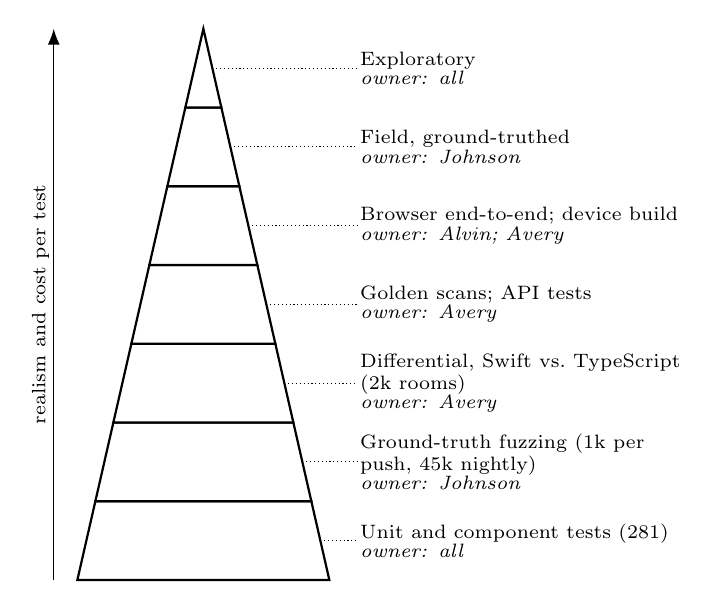
\begin{tikzpicture}[font=\scriptsize]
  \def\H{7.0} \def\W{1.6} \def\LX{1.95}
  \foreach \i/\lab/\own in {
      0/{Unit and component tests (281)}/{all},
      1/{Ground-truth fuzzing (1k per push, 45k nightly)}/{Johnson},
      2/{Differential, Swift vs.\ TypeScript (2k rooms)}/{Avery},
      3/{Golden scans; API tests}/{Avery},
      4/{Browser end-to-end; device build}/{Alvin; Avery},
      5/{Field, ground-truthed}/{Johnson},
      6/{Exploratory}/{all}} {
    \pgfmathsetmacro{\yb}{\i*\H/7}
    \pgfmathsetmacro{\yt}{(\i+1)*\H/7}
    \pgfmathsetmacro{\xb}{\W*(1-\yb/\H)}
    \pgfmathsetmacro{\xt}{\W*(1-\yt/\H)}
    \pgfmathsetmacro{\ym}{(\yb+\yt)/2}
    \pgfmathsetmacro{\xm}{(\xb+\xt)/2}
    \draw[thick, fill=white] (-\xb,\yb) -- (\xb,\yb) -- (\xt,\yt) -- (-\xt,\yt) -- cycle;
    \draw[densely dotted] (\xm,\ym) -- (\LX,\ym);
    \node[anchor=west, align=left, text width=4.15cm, inner sep=1pt] at (\LX,\ym)
      {\lab\\[-1pt]\textit{owner: \own}};
  }
  \draw[-{Latex[length=2mm]}] (-\W-0.3,0) -- node[rotate=90, above, inner sep=1.5pt]
    {realism and cost per test} (-\W-0.3,\H);
\end{tikzpicture}
\caption{Test levels, from fast and numerous (bottom) to realistic and costly
(top), with the owner of each level.}
\label{fig:pyramid}
\end{figure}

\begin{table*}[!t]
\caption{Test Levels, Techniques, Oracles and Owners}
\label{tab:levels}
\centering
\footnotesize
\begin{tabularx}{\textwidth}{@{}L{2.5cm}L{3.2cm}YL{1.9cm}L{1.6cm}L{2.0cm}@{}}
\toprule
Level & Objective & Technique and oracle & Tooling & Owner & Runs \\
\midrule
Unit and component & functions behave as specified & example-based assertions & Vitest~\cite{vitest} & all & every push \\
Ground-truth fuzzing & outline correct on realistic rooms & generated rooms with known outline; oracle (\ref{eq:oracle}) & seeded generator & Johnson & push (1k); nightly (45k) \\
Differential testing & Swift and TypeScript agree & identical inputs to both; tolerance (\ref{eq:parity}) & Swift harness & Avery & every push \\
Golden-scan regression & real scans import unchanged & snapshot comparison; reviewed diffs & Vitest & Avery & every push \\
API and integration & handoff contract and error paths & request--response assertions; fault injection & HTTP client & Avery & every push \\
Browser end-to-end & user flows work in a browser & scripted interaction with a production build & Playwright~\cite{playwright} & Alvin & every push \\
Visual regression & plan and 3D unchanged unless intended & screenshot difference with threshold & Playwright & Alvin & every push (from week 3) \\
Device build & the whole app compiles & unsigned \texttt{xcodebuild} & Xcode (CI) & Avery & every push \\
Field & accuracy in real rooms & ground truth and scoring (Section~\ref{sec:criteria}) & laser meter; scoring tool & Johnson & every session \\
Exploratory & unanticipated failures & time-boxed charters & --- & all & weekly \\
Performance & detection time; frame rate; latency & measurement against limits & on-device log; load tool & Johnson; Alvin; Avery & weekly \\
Security and abuse & misuse and privacy & malformed input; code guessing; retention & HTTP fuzzing & Avery & week 3 \\
\bottomrule
\end{tabularx}
\end{table*}

\subsection{Ground-truth fuzzing}

The wall analysis is tested in the style of property-based
testing~\cite{quickcheck}. A seeded generator produces rooms whose true
outline is known, and then degrades each room the way a furnished room
degrades a scan. Four families of floor plan are drawn: rectangular, L-shaped,
U-shaped, and irregular rooms with five to seven walls at arbitrary angles.
Each is placed at a random rotation and position. Each wall is split into up
to three fragments, with gaps of up to 600\,mm and insets of up to 180\,mm
into the room. Low clutter is placed in front of some walls, and round or
square pillars are placed in some rooms. With $V$ the produced outline
vertices, $V^{\ast}$ the true ones and $A$, $A^{\ast}$ their areas, an
outline is accepted if
\begin{equation}
d_H(V,V^{\ast}) \le 5\,\text{mm} \quad\text{and}\quad
\frac{|A-A^{\ast}|}{A^{\ast}} \le 0.002,
\label{eq:oracle}
\end{equation}
where $d_H$ is the symmetric Hausdorff distance between the two vertex sets.
The oracle therefore penalises corners that are missed as well as corners
that are invented. Seeding makes every failure reproducible from its seed
and index. This level found the U-shaped-room defects that the hand-written
cases had not reached (Section~\ref{sec:results}).

\subsection{Differential testing}\label{sec:differential}

The iPad runs Swift, while most tests are written in TypeScript. A small
harness compiles the app's own Swift sources and runs them on exactly the
inputs that the TypeScript test generates: rooms, glass cases and camera
images. Each numerical output $x_S$ of the Swift code and $x_T$ of the
TypeScript code must satisfy
\begin{equation}
|x_S - x_T| \le 10^{-6}\,\max(1, |x_T|).
\label{eq:parity}
\end{equation}
This is differential testing in the sense of McKeeman~\cite{mckeeman}. It
establishes that the two implementations are equivalent, not that either is
correct. Correctness comes from the unit, fuzzing and field levels.

\subsection{Golden-scan regression}

Each scored field scan is stored alongside a snapshot of what the web makes
of it: walls, area, openings, columns, furniture and fixtures. Any change in
that output fails the build and shows up as a reviewable difference. A
snapshot may only be updated with a written justification. This is how a
defect found in one room stays fixed in every later build.

\subsection{Field protocol}\label{sec:field}

\textbf{Ground truth.} Before a room is scanned, it is measured with a laser
distance meter ($\pm$2\,mm). Every wall is measured corner to corner at floor
level, behind the furniture. The ceiling height is the median of three
readings. Each column's diameter (or wider face) is measured; doors and
windows are counted, with glass panes and mirrors noted; and every socket is
inventoried by wall, offset and height, with a photograph.

\textbf{Scanning.} Each scan follows the same walk: clockwise, 1--1.5\,m from
the walls, passing each wall twice and moving sideways past each socket. The
detection time shown on screen is recorded at the start, middle and end.
After the scan, the tester reviews glass suggestions, removes the furniture
and adds any missed openings. Every correction is recorded, because the
number of corrections measures the friction a customer would face. Each room
is scanned three times, by two testers where possible.

\textbf{Scoring.} Testers list walls in order from an arbitrary corner, in
either direction, so the $n$ scanned lengths $\hat\ell$ are aligned with the
measured lengths $\ell$ by
\begin{equation}
\pi^{\ast} = \arg\min_{r\in\{0,\dots,n-1\},\; s\in\{\pm1\}}\;
\max_i \bigl|\hat\ell_{(r+s\,i)\bmod n}-\ell_i\bigr|,
\label{eq:align}
\end{equation}
and wall $i$ passes if
$|\hat\ell_{\pi^{\ast}(i)}-\ell_i| \le \max(30\,\text{mm},\,0.015\,\ell_i)$.
The scoring tool applies this rule and every other limit in
Table~\ref{tab:criteria}, and prints a pass/fail table for each scan.

\textbf{Sample size.} Socket recall
$R = \mathit{TP}/(\mathit{TP}+\mathit{FN})$ and precision
$P = \mathit{TP}/(\mathit{TP}+\mathit{FP})$ are reported with Wilson 95\%
intervals~\cite{wilson}. Showing recall $\ge 0.90$ at 95\% confidence means
the lower bound must reach 0.90. With no misses at all this requires
35~sockets; with 80~sockets it tolerates at most two misses. The campaign
therefore inventories at least 80~sockets across its rooms. The per-room
point estimate is used for acceptance, and the interval is reported alongside
it.

\subsection{Exploratory testing}

Scripted cases check what was anticipated. Three charters of 30 minutes each,
run weekly, look for what was not:
\begin{itemize}
\item \emph{break the floor plan}: unusual rooms, stairs, half-open doors,
  scanning too fast, starting in the middle of the room;
\item \emph{lighting torture}: dusk, every lamp on, a television playing,
  flickering LEDs, a torch;
\item \emph{handoff abuse}: two iPads sending at once, a room re-sent after
  editing, a code opened on a phone.
\end{itemize}

% =============================================================================
\section{Test Environment}\label{sec:env}

\subsection{Devices, software and tools}

\begin{table}[!t]
\caption{Test Environment}
\label{tab:env}
\centering
\footnotesize
\begin{tabularx}{\columnwidth}{@{}L{1.9cm}Y@{}}
\toprule
Item & Configuration \\
\midrule
iPad A & iPad Pro with LiDAR, M1 generation or earlier; iPadOS 17 \\
iPad B & iPad Pro (M4); current iPadOS \\
iPad builds & Debug with optimisation (field sessions); TestFlight release candidate (week 4) \\
Browsers & Chrome, Safari (macOS), Safari (iPadOS), Edge; current versions \\
CI & GitHub Actions: Ubuntu (web, parity, nightly fuzzing); macOS~15 (device build) \\
Backend & local (in-memory store); staging and production (shared key--value store, 24\,h expiry) \\
Measurement & laser distance meter ($\pm$2\,mm); 5\,m tape; camera \\
\bottomrule
\end{tabularx}
\end{table}

Table~\ref{tab:env} lists the environment. Two iPads of different generations
are used, so that performance limits are tested on the slowest device likely
to be in customers' hands.

\subsection{Room matrix}

Table~\ref{tab:rooms} lists the room types the campaign must find. Rooms marked
\req{} are required; the release is blocked without a passing result in each.

\begin{table}[!t]
\caption{Room Matrix (\req{} required for release)}
\label{tab:rooms}
\centering
\footnotesize
\begin{tabularx}{\columnwidth}{@{}L{0.55cm}L{2.5cm}YC{0.35cm}@{}}
\toprule
ID & Room & Exercises & \\
\midrule
R1 & plain rectangle & baseline accuracy & \req \\
R2 & L-shaped & reflex corner & \req \\
R3 & U-shaped or notched & notch kept, not bridged & \req \\
R4 & free-standing round column & circle fit; no spike & \req \\
R5 & square or engaged column & box; wall stays straight & \req \\
R6 & sliding glass door & glass suggestion (door) & \req \\
R7 & full-height window & glass suggestion (window) & \req \\
R8 & large mirror & negative control for glass & \req \\
R9 & LED strips, downlights & light rejection; recall & \req \\
R10 & shoes, boxes along a wall & clutter rejection & \req \\
R11 & sunlit socket wall & clipped plates kept & \\
R12 & attic or knee wall & low wall kept & \\
R13 & rounded corner & no false column & \\
R14 & open plan over 8\,m & long walls; drift & \\
R15 & whole flat, three or more rooms & multi-room session & \req \\
\bottomrule
\end{tabularx}
\end{table}

% =============================================================================
\section{Acceptance Criteria}\label{sec:criteria}

Table~\ref{tab:criteria} gives the limits that each scan is held to. They are
encoded in the scoring tool (\code{scripts/scan-accuracy.mjs}), so a field
session ends with numbers rather than impressions.

\begin{table}[!t]
\caption{Acceptance Limits}
\label{tab:criteria}
\centering
\footnotesize
\begin{tabularx}{\columnwidth}{@{}L{2.4cm}Y@{}}
\toprule
Measure & Limit \\
\midrule
Wall length & $\pm$30\,mm or $\pm$1.5\%, whichever is larger \\
Floor area & $\pm$2\% \\
Ceiling height & $\pm$30\,mm \\
Wall, column, opening counts & exact (openings after review of glass suggestions) \\
Column size & $\pm$40\,mm \\
Socket recall & $\ge$ 0.90 per room; $\ge$ 0.95 overall \\
Socket precision & $\ge$ 0.95 (at most one false socket per two rooms) \\
Glass recall & $\ge$ 0.80 of unrecognised panes suggested \\
Detection time & $\le$ 150\,ms per frame (median); $\le$ 300\,ms (95th percentile) \\
Stability & no crash in the last 20 scans before release \\
Handoff & every code opens the same room on the web \\
\bottomrule
\end{tabularx}
\end{table}

\textbf{Release criteria.} The release candidate ships only if all of the
following hold:
\begin{enumerate}
\item there is no open defect of severity P0;
\item there is no open P1 defect in a required room;
\item the limits of Table~\ref{tab:criteria} are met in at least 90\% of
  release-candidate scans of required rooms;
\item every CI job is green; and
\item at least ten scans by people outside the team were completed without
  assistance.
\end{enumerate}

% =============================================================================
\section{Schedule}\label{sec:schedule}

The plan runs for four working weeks, from Monday 5 to Friday 30 October
2026. Fig.~\ref{fig:gantt} shows the workstreams of each owner, and
Table~\ref{tab:weeks} states each week's objective, the work of each owner and
the milestone that closes the week. A milestone is met only when its exit
criterion is satisfied. Otherwise the shortfall is carried into the next week
as a P1 defect.

\begin{figure*}[!t]
\centering
\resizebox{\textwidth}{!}{%
\begin{ganttchart}[
    hgrid={*4{draw=none}, *1{dotted}},
    vgrid={*4{densely dotted}, *1{solid}},
    x unit=0.62cm,
    y unit title=0.42cm,
    y unit chart=0.36cm,
    title/.append style={draw=black, fill=white},
    title label font=\footnotesize,
    bar label font=\footnotesize,
    group label font=\footnotesize\bfseries,
    milestone label font=\footnotesize\itshape,
    bar height=0.6,
    group height=0.25,
    group peaks height=0.15,
    group/.append style={fill=black},
    milestone/.append style={fill=black},
    johnson/.style={bar/.append style={fill=black}},
    avery/.style={bar/.append style={pattern=north east lines}},
    alvin/.style={bar/.append style={fill=white}},
  ]{1}{20}
  \gantttitle{Week 1 (5--9 Oct)}{5}
  \gantttitle{Week 2 (12--16 Oct)}{5}
  \gantttitle{Week 3 (19--23 Oct)}{5}
  \gantttitle{Week 4 (26--30 Oct)}{5} \\
  \gantttitle{M}{1} \gantttitle{T}{1} \gantttitle{W}{1} \gantttitle{T}{1} \gantttitle{F}{1} \gantttitle{M}{1} \gantttitle{T}{1} \gantttitle{W}{1} \gantttitle{T}{1} \gantttitle{F}{1} \gantttitle{M}{1} \gantttitle{T}{1} \gantttitle{W}{1} \gantttitle{T}{1} \gantttitle{F}{1} \gantttitle{M}{1} \gantttitle{T}{1} \gantttitle{W}{1} \gantttitle{T}{1} \gantttitle{F}{1} \\
  \ganttgroup{Johnson -- scanning}{1}{20} \\
  \ganttbar[johnson]{Raw-surface export; build label}{1}{3} \\
  \ganttbar[johnson]{Field round 1 (R1, R2, R4, R6, R9, R10)}{2}{5} \\
  \ganttbar[johnson]{Fixes, XCTest target, on-device timing}{6}{9} \\
  \ganttbar[johnson]{Field round 2 (R3, R5, R7, R8, R11--R13)}{7}{10} \\
  \ganttbar[johnson]{R14, R15, stress scan, lighting charter}{11}{15} \\
  \ganttbar[johnson]{RC regression on device; external beta}{17}{20} \\
  \ganttgroup{Avery -- backend}{1}{20} \\
  \ganttbar[avery]{CI live; device build green}{1}{2} \\
  \ganttbar[avery]{API tests; staging with shared store}{3}{5} \\
  \ganttbar[avery]{Golden corpus; weekly scoring report}{6}{10} \\
  \ganttbar[avery]{SDK and schema compatibility tests}{8}{10} \\
  \ganttbar[avery]{Hardening, rate limits, load test}{11}{15} \\
  \ganttbar[avery]{Production deployment; monitoring}{16}{20} \\
  \ganttgroup{Alvin -- front end}{1}{20} \\
  \ganttbar[alvin]{End-to-end in CI; manual web pass}{1}{5} \\
  \ganttbar[alvin]{Placement and orientation; recommender}{6}{10} \\
  \ganttbar[alvin]{Visual regression harness}{8}{13} \\
  \ganttbar[alvin]{WebKit; cross-browser; performance}{11}{15} \\
  \ganttbar[alvin]{Web RC regression; beta support}{16}{20} \\
  \ganttgroup{Milestones}{1}{20} \\
  \ganttmilestone{M1: CI green; 18 scans scored}{5} \\
  \ganttmilestone{M2: accuracy limits met}{10} \\
  \ganttmilestone{M3: every case run; P1 under control}{15} \\
  \ganttmilestone{M4: go/no-go decision}{20}
\end{ganttchart}}
\caption{Schedule by owner. Solid bars: Johnson (scanning); hatched bars:
Avery (backend); outlined bars: Alvin (front end). Diamonds mark the weekly
milestones M1--M4. Code freeze is on Tuesday 27 October.}
\label{fig:gantt}
\end{figure*}

\begin{table*}[!t]
\caption{Weekly Objectives, Division of Work and Exit Criteria}
\label{tab:weeks}
\centering
\footnotesize
\begin{tabularx}{\textwidth}{@{}L{1.9cm}YYYL{3.3cm}@{}}
\toprule
Week & Johnson (scanning) & Avery (backend) & Alvin (front end) & Exit criterion \\
\midrule
1: make results trustworthy (5--9 Oct) &
Measuring kit and tester training; raw-surface export; build label on
screen; field round 1, six rooms $\times$ 3 scans, scored and logged. &
CI live with all jobs; first device build made green with Johnson and
Alvin; API cases automated; staging with shared store; round-1 scans
ingested as golden scans. &
End-to-end suite in CI; manual pass of WEB-01 to WEB-08 in Chrome; model
audit script; design-mode compile fixes. &
\textbf{M1}: all CI jobs green; 18 field scans scored. \\
\addlinespace
2: accuracy (12--16 Oct) &
Week-1 defects fixed test-first; XCTest target; on-device timing log;
socket detector tuned on field images; field round 2 (required rooms
complete). &
Golden corpus of at least ten real rooms, enforced where passing; automated
weekly scoring report; SDK round-trip and schema tests; concurrency and
multi-instance tests. &
Placement and orientation verified on real scans; recommender validity;
visual regression harness started; design-mode comparison with web. &
\textbf{M2}: required rooms measured; walls pass in $\ge$90\% of scans;
socket recall $\ge$ 0.90; no P0. \\
\addlinespace
3: robustness (19--23 Oct) &
Open plan and whole flat; ten-minute stress scan on both iPads; lighting
charter; review of the glass-versus-mirror interaction. &
Expiry and retry behaviour; rate-limit decision; load test; render-proxy
timeouts; monitoring of the handoff store. &
WebKit end-to-end; cross-browser matrix; frame-rate and accessibility
passes; visual regression in CI. &
\textbf{M3}: every case run once; at most two P1, none in a required room. \\
\addlinespace
4: release candidate (26--30 Oct) &
Code freeze Tuesday; TestFlight build; full device regression; external
beta of 3--5 people and at least ten scans; final metrics; chairs go/no-go. &
Production deployment of the handoff; backend regression; monitoring
during the beta; verification of 24-hour retention. &
Web regression on the release candidate in every browser; final visual
baselines; support of the web half of the beta. &
\textbf{M4}: release criteria of Section~\ref{sec:criteria} met;
decision recorded. \\
\bottomrule
\end{tabularx}
\end{table*}

% =============================================================================
\section{Risks and Mitigations}\label{sec:risks}

Table~\ref{tab:risks} lists the principal risks, each with a likelihood (L),
an impact (I) and an owner. The first risk is scheduled for the first day
because it can block everything else: the iPad's interface code has been
reviewed but has never been compiled by Xcode in CI.

\begin{table*}[!t]
\caption{Risk Register (H high, M medium, L low)}
\label{tab:risks}
\centering
\footnotesize
\begin{tabularx}{\textwidth}{@{}L{0.5cm}L{5.4cm}C{0.35cm}C{0.35cm}YL{2.3cm}@{}}
\toprule
\# & Risk & L & I & Mitigation & Owner \\
\midrule
1 & Interface code fails to compile in Xcode, blocking device testing & M & H & device-build job on day 1; fixes paired across owners & Avery (pipeline); Johnson, Alvin \\
2 & Real rooms break the wall analysis in ways generated rooms do not & M & H & raw-surface export; field scans replayed as tests & Johnson \\
3 & Mirrors suggested as glass & H & L & one-tap removal; counted in metrics; interaction reviewed in week 3 & Johnson \\
4 & Socket recall below target under real lighting & M & H & tuning on field images; at least 80 sockets inventoried & Johnson \\
5 & Older iPads too slow for detection & M & M & per-device timing; adaptive sampling; candidate cap & Johnson \\
6 & In-memory store deployed on several instances, so codes are not found & M & H & staging with shared store; startup warning; multi-instance test & Avery \\
7 & Codes guessed, exposing room layouts (no rate limit at baseline) & L & H & rate-limit decision; 24\,h expiry; enumeration test & Avery \\
8 & Long renders cut off by proxy or hosting timeouts & M & M & timeout tests; documented limits & Avery \\
9 & Web models differ from the iPad's USDZ & L & M & audit of every catalogue model & Alvin \\
10 & Safari-specific rendering or input defects & M & M & WebKit end-to-end; manual iPad Safari pass & Alvin \\
11 & Required room types not available for the field campaign & M & M & rooms identified in week 1; showroom fallback & Johnson \\
12 & Swift and TypeScript implementations drift apart & L & H & differential job blocks merging & Avery \\
13 & A newer schema version is silently read as version 1 (no version check at baseline) & L & M & version check in the parser; test SDK-02 & Avery \\
\bottomrule
\end{tabularx}
\end{table*}

% =============================================================================
\section{Defect Management and Reporting}\label{sec:defects}

\subsection{Severity}

\begin{table}[!t]
\caption{Defect Severity and Response}
\label{tab:severity}
\centering
\footnotesize
\begin{tabularx}{\columnwidth}{@{}L{0.8cm}YL{2.3cm}@{}}
\toprule
Level & Definition & Response \\
\midrule
P0 & crash, data loss, scan cannot be completed, or a code opens the wrong room & same or next day; blocks release \\
P1 & a required room outside the limits; a feature unusable & within the week; blocks release \\
P2 & wrong but correctable in one or two taps & scheduled \\
P3 & cosmetic or wording & backlog \\
\bottomrule
\end{tabularx}
\end{table}

Table~\ref{tab:severity} defines the severity levels and the expected
response to each.

\subsection{Workflow}

\begin{enumerate}
\item \emph{Report} the defect with the issue template, attaching the scan
  file and, for field defects, the room's ground truth.
\item \emph{Triage} at the daily meeting, which assigns a severity and an
  owner within one working day.
\item \emph{Reproduce} the defect from the attached scan, as a failing
  automated test: a golden scan, a raw-surface replay, a detector image or an
  end-to-end step.
\item \emph{Fix} the defect, get CI green, and \emph{verify} the fix on a
  device in the same room before closing the issue.
\end{enumerate}

\subsection{Weekly report}

The Friday report contains the following metrics, each with its owner:
\begin{itemize}
\item rooms tested against rooms required (Johnson);
\item wall pass rate and wall error at the 50th and 95th percentiles
  (Johnson, using Avery's tooling);
\item socket recall and precision, with Wilson intervals (Johnson);
\item glass panes suggested, real and kept; corrections per scan (Johnson);
\item detection time per device; crashes (Johnson);
\item handoff error rate and latency; CI pass rate; nightly fuzzing failures
  (Avery);
\item end-to-end and visual-regression results; browser matrix (Alvin);
\item open defects by severity (all).
\end{itemize}

% =============================================================================
\section{Preliminary Results}\label{sec:results}

Table~\ref{tab:results} records the evidence available at the baseline commit
before the campaign starts. The automated levels are in place and passing. The
two levels that can only be completed with hardware have not yet run: the
device build and field accuracy.

\begin{table}[!t]
\caption{Evidence at the Baseline (1 October 2026)}
\label{tab:results}
\centering
\footnotesize
\begin{tabularx}{\columnwidth}{@{}YL{2.45cm}@{}}
\toprule
Evidence & Result \\
\midrule
Unit and component tests & 281 passed, 0 failed \\
Fuzzing, previous build, 1{,}000 rooms & 278 incorrect outlines \\
Fuzzing, baseline, 1{,}000 rooms & 0 incorrect \\
Fuzzing, baseline, two runs of 15{,}000 rooms & 6 and 9 incorrect (0.04\%, 0.06\%) \\
Differential, 2{,}000 rooms, 100 glass cases, 7 images & 0 disagreements \\
Browser end-to-end (Chromium) & 8 of 8 passed \\
Device build (Xcode, full app) & not yet run \\
Field accuracy (Table~\ref{tab:criteria}) & not yet measured \\
\bottomrule
\end{tabularx}
\end{table}

The drop from 278 to 0 incorrect outlines out of 1{,}000 reflects defects
that fuzzing found and that have since been fixed. A notch in a U-shaped room
was bridged when one of its walls arrived in pieces. Inside corners and
rounded corners were taken for columns. A pillar was judged against an
outline that had lost one of its own corners. Clutter was judged only against
the visible parts of the wall it hid. The residue at 15{,}000 rooms falls
almost entirely in U-shaped rooms. Its root cause is open and assigned to
Johnson in week~2. Meanwhile it is tracked nightly against a budget of 0.1\%.

\subsection{Threats to validity}

\emph{Generator realism.} The generated defects model our understanding of
RoomPlan's errors, not RoomPlan itself. The raw-surface export and the field
corpus exist to close this gap.
\emph{Equivalence is not correctness.} Differential testing shows that the
two implementations agree; the other levels must show that they are right.
\emph{Single browser engine.} Until week~3, end-to-end tests run only in
Chromium.
\emph{Sample size.} A few dozen rooms cannot estimate rare failures. Nightly
fuzzing covers rarity and the field covers realism; neither substitutes for
the other.
\emph{Tester effects.} Two testers and a standard walk limit, but do not
remove, the influence of scanning technique.

% =============================================================================
\section{Conclusion}\label{sec:conclusion}

This plan assigns the verification of MOZU's scan-to-design pipeline to three
owners, along the boundaries of the system itself. Johnson owns the scan,
Avery the services and data between the devices, and Alvin everything the
user sees on the web. It makes every claim measurable: field results are
scored against fixed limits, and automated evidence is produced on every
change. The automated evidence is already strong for the geometry, at 0
incorrect outlines in 1{,}000 rooms and exact agreement between the two
implementations, but it says nothing yet about real LiDAR in real rooms.
Weeks 1 and 2 supply that evidence, week 3 hardens the system, and week 4
decides on release against criteria fixed in advance.

% =============================================================================
% Balance the last two-column page: the references start the right-hand
% column. Remove this \newpage if the text above changes length so much that
% the conclusion no longer ends in the left-hand column of that page.
\newpage

\begin{thebibliography}{99}

\bibitem{ieee829}
\emph{IEEE Standard for Software and System Test Documentation}, IEEE Std
829-2008, 2008.

\bibitem{iso29119}
\emph{Software and Systems Engineering---Software Testing---Part 3: Test
Documentation}, ISO/IEC/IEEE 29119-3:2021, 2021.

\bibitem{roomplan}
Apple Inc., ``RoomPlan,'' Apple Developer Documentation. [Online]. Available:
\url{https://developer.apple.com/documentation/roomplan}

\bibitem{ardepth}
Apple Inc., ``ARDepthData,'' ARKit, Apple Developer Documentation. [Online].
Available: \url{https://developer.apple.com/documentation/arkit/ardepthdata}

\bibitem{kasa}
I.~K{\aa}sa, ``A circle fitting procedure and its error analysis,''
\emph{IEEE Trans. Instrum. Meas.}, vol.~IM-25, no.~1, pp.~8--14, Mar. 1976.

\bibitem{quickcheck}
K.~Claessen and J.~Hughes, ``QuickCheck: A lightweight tool for random testing
of Haskell programs,'' in \emph{Proc. 5th ACM SIGPLAN Int. Conf. Functional
Programming (ICFP)}, 2000, pp.~268--279.

\bibitem{mckeeman}
W.~M. McKeeman, ``Differential testing for software,'' \emph{Digital
Technical Journal}, vol.~10, no.~1, pp.~100--107, 1998.

\bibitem{cohn}
M.~Cohn, \emph{Succeeding with Agile: Software Development Using Scrum}.
Upper Saddle River, NJ, USA: Addison-Wesley, 2009.

\bibitem{wilson}
E.~B. Wilson, ``Probable inference, the law of succession, and statistical
inference,'' \emph{J. Amer. Statist. Assoc.}, vol.~22, no.~158,
pp.~209--212, 1927.

\bibitem{playwright}
Microsoft, ``Playwright.'' [Online]. Available: \url{https://playwright.dev}

\bibitem{vitest}
Vitest contributors, ``Vitest.'' [Online]. Available:
\url{https://vitest.dev}

\end{thebibliography}

% =============================================================================
%  Appendices — one column, so the catalogue can run across pages
% =============================================================================
\onecolumn
\appendices

\section{Test-Case Catalogue}\label{app:cases}

Priority (P): H must pass for release; M should pass; L informative. Room
identifiers refer to Table~\ref{tab:rooms}; limits to
Table~\ref{tab:criteria}.

\setlength{\LTpre}{4pt}
\setlength{\LTpost}{6pt}
\footnotesize

\subsection{Johnson --- scanning (iPad, field)}\label{app:johnson}

\begin{longtable}{@{}L{1.25cm}L{3.6cm}L{5.4cm}L{5.1cm}C{0.4cm}@{}}
\toprule
ID & Test case & Procedure & Expected result & P \\
\midrule
\endhead
\bottomrule
\endfoot
SCN-01 & Baseline accuracy & Scan R1 by the standard walk; score it. & All wall, area and ceiling checks pass. & H \\
SCN-02 & Non-convex rooms & Scan R2 and R3. & Wall count exact; reflex corner and notch present. & H \\
SCN-03 & Repeatability & Three scans of one room by two testers. & Wall lengths agree within $\pm$20\,mm. & H \\
SCN-04 & Clutter along a wall & R10: shoes and boxes along 1.5\,m of wall. & Wall straight; within the wall limit. & H \\
SCN-05 & Low furniture & R10: shoe rack 40--90\,cm tall against a wall. & Not drawn as a wall. & H \\
SCN-06 & Knee wall & Scan R12. & Low wall kept in the outline. & M \\
COL-01 & Round column & Scan R4. & One round column, drawn as a circle, size within limit; no spike. & H \\
COL-02 & Square or engaged column & Scan R5. & Box column; adjoining wall straight. & H \\
COL-03 & Rounded corner & Scan R13. & Corner stays in the walls; no column reported. & M \\
COL-04 & Columns survive & Furniture $\rightarrow$ Remove all. & Columns remain. & H \\
GLS-01 & Glass door & R6: look at the door for about 3\,s during the walk. & Dashed suggestion on that wall; review banner shown. & H \\
GLS-02 & Large window & Scan R7. & Window suggestion; sill within 100\,mm. & H \\
GLS-03 & Review persists & Keep one suggestion, remove another, send to web. & Kept as opening; removed absent; same on web. & H \\
GLS-04 & Mirror & Scan R8. & A suggestion is acceptable; removed in one tap. & M \\
OPN-01 & Add an opening & Windows $\rightarrow$ tap a bare wall; set width, height, sill. & Added at the tap; values held to wall and ceiling. & H \\
OPN-02 & Slide an opening & Drag an opening past the end of its wall. & Stops at the corner. & M \\
OPN-03 & Window sill & Compare a recognised window's sill with the measurement. & Within 50\,mm. & H \\
SKT-01 & Socket recall & R1: walk past every socket sideways. & Recall $\ge$ 0.90; no false sockets. & H \\
SKT-02 & Lights are not sockets & R9: LED strips and downlights in view for 30\,s. & No markers on any light. & H \\
SKT-03 & Socket under a light & R9: socket directly beneath an LED strip. & Socket confirmed. & H \\
SKT-04 & Marker stability & Pan across a confirmed socket. & Marker stays on it; number unchanged. & H \\
SKT-05 & Pinned socket & Pin a socket by hand; keep scanning past it. & Pin does not move. & M \\
SKT-06 & Sunlit socket & Scan R11. & Socket detected. & M \\
SKT-07 & Double socket & Two outlets side by side. & Two markers. & H \\
SKT-08 & Socket height & Compare plan heights with the inventory. & Within 50\,mm. & H \\
FUR-01 & Remove furniture & Furniture $\rightarrow$ select $\rightarrow$ Remove; then Remove all. & Removed; Done always available; editor closes when empty. & H \\
PRF-01 & Detection time & Read the time per frame in every scan, on both iPads. & Within the limits of Table~\ref{tab:criteria}. & H \\
PRF-02 & Endurance & Ten-minute scan of R15. & No crash or thermal shutdown; markers smooth. & H \\
DEV-01 & Swift unit tests & Run the XCTest target. & All pass on device and in CI. & M \\
DEV-02 & Field replay & Export raw surfaces from a failing field scan; replay. & The failure reproduces as an automated test. & H \\
\end{longtable}

\subsection{Avery --- backend (services, data, CI)}\label{app:avery}

\begin{longtable}{@{}L{1.25cm}L{3.6cm}L{5.4cm}L{5.1cm}C{0.4cm}@{}}
\toprule
ID & Test case & Procedure & Expected result & P \\
\midrule
\endhead
\bottomrule
\endfoot
API-01 & Create a code & POST a valid scan. & 201; six characters from the 30-symbol alphabet; URL; expiry 24\,h ahead. & H \\
API-02 & Round trip & GET the scan by its code. & Deep-equal to the scan sent. & H \\
API-03 & Forgiving entry & Lower case, spaces, hyphens, confusable characters (O/0, I/L/1, U). & Normalised to the same code. & H \\
API-04 & Unknown or expired code & GET a code never issued, and one past expiry. & 404; no data returned. & H \\
API-05 & Missing code & GET without a code. & 400. & M \\
API-06 & Oversize payload & POST more than 2{,}000{,}000 bytes. & 413 with the limit stated. & H \\
API-07 & Malformed input & POST invalid JSON; then valid JSON that is not a RoomScan. & 400; then 422. & H \\
API-08 & Store unavailable & Fault-inject a store failure. & 503 with a retryable message; the iPad shows it and retries. & H \\
API-09 & Expiry & Advance a fake clock past 24\,h. & Entry no longer readable; removed by the sweep. & H \\
API-10 & Concurrency & 100 parallel uploads. & 100 distinct codes; no cross-talk between payloads. & H \\
API-11 & Multiple instances & Staging with two instances and a shared store. & A code created on one instance is readable on the other. & H \\
SEC-01 & Code guessing & 10{,}000 random code requests. & No hits; requests throttled once rate limiting is decided. & M \\
SEC-02 & Retention & Inspect the store 24\,h after upload. & No scan data retained. & M \\
SDK-01 & Serialisation & Random scans through serialise and parse. & Identical after the round trip. & H \\
SDK-02 & Schema compatibility & Scans lacking optional fields; scans with unknown fields; a future schema version. & First two parse; the third is rejected with 422. At the baseline it is accepted and read as version 1, so this case is expected to fail until fixed. & H \\
SDK-03 & Deep link & Build and parse the \texttt{/scan} URL for a large room. & Round trip exact; within URL length limits. & M \\
GLD-01 & Golden regression & Run the golden-scan suite. & All snapshots match; changes justified in review. & H \\
GLD-02 & Corpus growth & Ingest each scored field scan. & Added within one working day. & M \\
CI-01 & Pipeline & Push a change. & Web, parity and device-build jobs green. & H \\
CI-02 & Nightly fuzzing & Inspect the nightly run of 45{,}000 rooms. & Within the 0.1\% budget; any excess raised. & M \\
REN-01 & Render proxy & No server; failing server; render longer than five minutes. & 503; 502; long render completes. & M \\
REN-02 & Render contents & Inspect a render request. & Modules, catalogue furniture and columns present; scanned furniture absent. & M \\
EST-01 & Estimate proxy & Missing key; malformed body; upstream failure. & 503; 400; 502. & L \\
LOAD-01 & Load & 50 requests per second, create and fetch, for 5 minutes on staging. & 95th-percentile latency below 300\,ms; no errors. & M \\
\end{longtable}

\subsection{Alvin --- front end (web 2D/3D, models, placement)}\label{app:alvin}

\begin{longtable}{@{}L{1.25cm}L{3.6cm}L{5.4cm}L{5.1cm}C{0.4cm}@{}}
\toprule
ID & Test case & Procedure & Expected result & P \\
\midrule
\endhead
\bottomrule
\endfoot
WEB-01 & Faithful import & Open a scan by code; compare with the iPad's plan. & Same walls, openings, columns; furniture in the same orientation. & H \\
WEB-02 & 2D and 3D agree & Drag and rotate furniture in 2D; inspect in 3D. & Same position and facing in both views. & H \\
WEB-03 & 3D drag & Drag an item across the floor in 3D. & Follows the pointer; held inside the room. & H \\
WEB-04 & Module placement & Drop a cabinet near a wall, then on open floor. & Seats against the wall facing the room; stays where dropped in the open. & H \\
WEB-05 & Selection & Select a window, then a sofa; press Delete. & The sofa is deleted, not the window. & H \\
WEB-06 & Opening inspector & Type 1500 into Width; enter a width larger than the wall. & 1500; held to the wall length. & H \\
WEB-07 & Columns & Drag, rotate or duplicate a column; raise the ceiling. & Not possible; column reaches the new ceiling. & H \\
WEB-08 & Height-only change & Change only the height; Apply. & Room shape, furniture and columns kept. & H \\
WEB-09 & Catalogue & Add each category's items. & Placed at the room centre; model loads, or blocks appear if it fails. & M \\
WEB-10 & Model fidelity & Compare every GLB with its USDZ. & Dimensions within 1\%; materials present. & M \\
WEB-11 & Recommender & Place each recommended set in R1--R3. & Inside the room; not through walls or columns; facing into the room. & M \\
WEB-12 & Finishes & Change colour of an item, the walls, floor and ceiling. & Applied in 3D and present in the render request. & H \\
WEB-13 & Lighting & Switch Studio, Daylight and Evening. & Renders without errors. & L \\
WEB-14 & Cross-browser & WEB-01 to WEB-08 in Safari (macOS), Safari (iPadOS) and Edge. & Same results as in Chrome. & H \\
WEB-15 & Performance & Twenty items in 3D on a typical laptop. & At least 30 frames per second; plan interactions under 100\,ms. & M \\
WEB-16 & Visual regression & Screenshot the plan and 3D view of every golden scan. & Differences only where intended. & M \\
WEB-17 & Accessibility & Keyboard navigation; labels on inputs; contrast. & Controls reachable and labelled. & L \\
WEB-18 & Design-mode parity & Open the same scan in the iPad's design mode and on the web. & Columns, orientation and finishes agree. & M \\
E2E-01 & Automated suite & Run the Playwright suite. & Green in Chromium; in WebKit from week 3. & H \\
\end{longtable}

\subsection{Joint integration cases (all three owners)}

\begin{longtable}{@{}L{1.25cm}L{3.6cm}L{5.4cm}L{5.1cm}C{0.4cm}@{}}
\toprule
ID & Test case & Procedure & Expected result & P \\
\midrule
\endhead
\bottomrule
\endfoot
INT-01 & Scan to web & Johnson scans and sends; Avery checks the stored payload; Alvin checks the web. & The same room at every stage. & H \\
INT-02 & Edits travel & Remove furniture, keep glass, add a window on the iPad; send. & All edits present on the web. & H \\
INT-03 & Whole flat & Scan R15 in one session; send. & Every room arrives, aligned in one coordinate frame. & H \\
INT-04 & Release regression & All high-priority cases on the release candidate. & Release criteria of Section~\ref{sec:criteria} met. & H \\
INT-05 & External beta & 3--5 people scan their own homes using only the written guide. & At least ten scans completed without assistance. & H \\
\end{longtable}

\normalsize

\section{Ground-Truth Record}\label{app:truth}

Each measured room is recorded in this form and scored with
\texttt{npm run scan:accuracy -- <scan.json> <truth.json>}. Walls are listed in
order round the room, from any corner, in either direction.

\begin{lstlisting}
{
  "room": "TPE-03 kitchen (tester initials, date)",
  "ciEnforce": false,
  "walls": [4210, 3405, 4205, 3410],
  "areaM2": 14.33,
  "ceilingMm": 2650,
  "columns": [{ "shape": "round", "diameterMm": 450 }],
  "openings": { "door": 1, "window": 2 },
  "sockets": 6
}
\end{lstlisting}

\section{Command Reference}\label{app:commands}

\begin{lstlisting}
npm run typecheck                  # application and SDK
npm test                           # unit, fuzzing (1,000 rooms), golden scans, scoring
npm run test:fuzz                  # 15,000 rooms
npm run test:parity                # Swift <-> TypeScript (needs a Swift toolchain)
npm run build && npm run test:e2e  # browser end-to-end
npm run test:golden:update         # after adding a scan to fixtures/scans
npm run scan:accuracy -- fixtures/scans/x.scan.json fixtures/scans/x.truth.json
\end{lstlisting}

\section{Document Control and Approval}\label{app:approval}

\begin{center}
\begin{tabular}{@{}ll@{}}
\toprule
Document & MOZU-TP-001, Test Plan \\
Version & 1.0 \\
Date & 1 October 2026 \\
Status & Issued for team review \\
Editor & Johnson \\
Distribution & Johnson, Avery, Alvin \\
\bottomrule
\end{tabular}

\vspace{14mm}

\begin{tabular}{@{}p{4.6cm}p{0.6cm}p{4.6cm}p{0.6cm}p{4.6cm}@{}}
\rule{4.6cm}{0.4pt} & & \rule{4.6cm}{0.4pt} & & \rule{4.6cm}{0.4pt} \\
Johnson, scanning lead & & Avery, backend lead & & Alvin, front-end lead \\[2pt]
Date: & & Date: & & Date: \\
\end{tabular}
\end{center}

\end{document}
